\documentclass{article}

\usepackage[utf8]{inputenc}
\usepackage[T1]{fontenc}
\usepackage[a4paper, margin=1in]{geometry}
\usepackage{amsmath}
\usepackage{graphicx}
\usepackage{listings}
\usepackage{xcolor}
\usepackage{tcolorbox}
\usepackage{scalerel}
\usepackage{bav4}


\title{Livrable 5}
\author{
Peran AMBERNY, Clement BARNOUIN, Loucas BURELLIER, \\
Vladimir KRAINIK--SAUL, Samuel SCHICKE 
}
\date{\today}

\begin{document}

\maketitle

\tableofcontents
\clearpage


\section{Introduction}
MiniCoffee est un groupe français spécialiste de l’univers du café, connu notamment pour ses machines à café en libre service. Pour l’année 2025, l’entreprise souhaite mettre à jour son infrastructure réseau interne en ajoutant : 
\begin{itemize}
    \item Divers serveurs d’utilité interne pour les employés et l'équipe informatique;
    \item Un réseau invité pour permettre à ses fournisseurs d’utiliser du matériel informatique sur place;
    \item Divers serveurs accessibles en ligne (site Web, serveur DNS public);
    \item Une meilleure communication entre ses machines à café et son infrastructure, qui a été un des points faibles de l’entreprise ces dernières années.
\end{itemize}
Pour cette tâche, MiniCoffee a fait appel à BAV4, notre équipe d’étudiants de l’IUT2 Informatique de Grenoble.

\section{Architecture}
L'architecture de notre réseau n'a pas énormément changé. 
Les seules modifications apportées au réseau sont : 
\begin{itemize}
    \item Passage d'un LAN à un VLAN pour une meilleure segmentation du réseau.
    \item Les adresses IP internes se terminent par 1XX.
    \item Les adresses IP externes se terminent par XX.
\end{itemize}

\begin{figure}
    \centering
    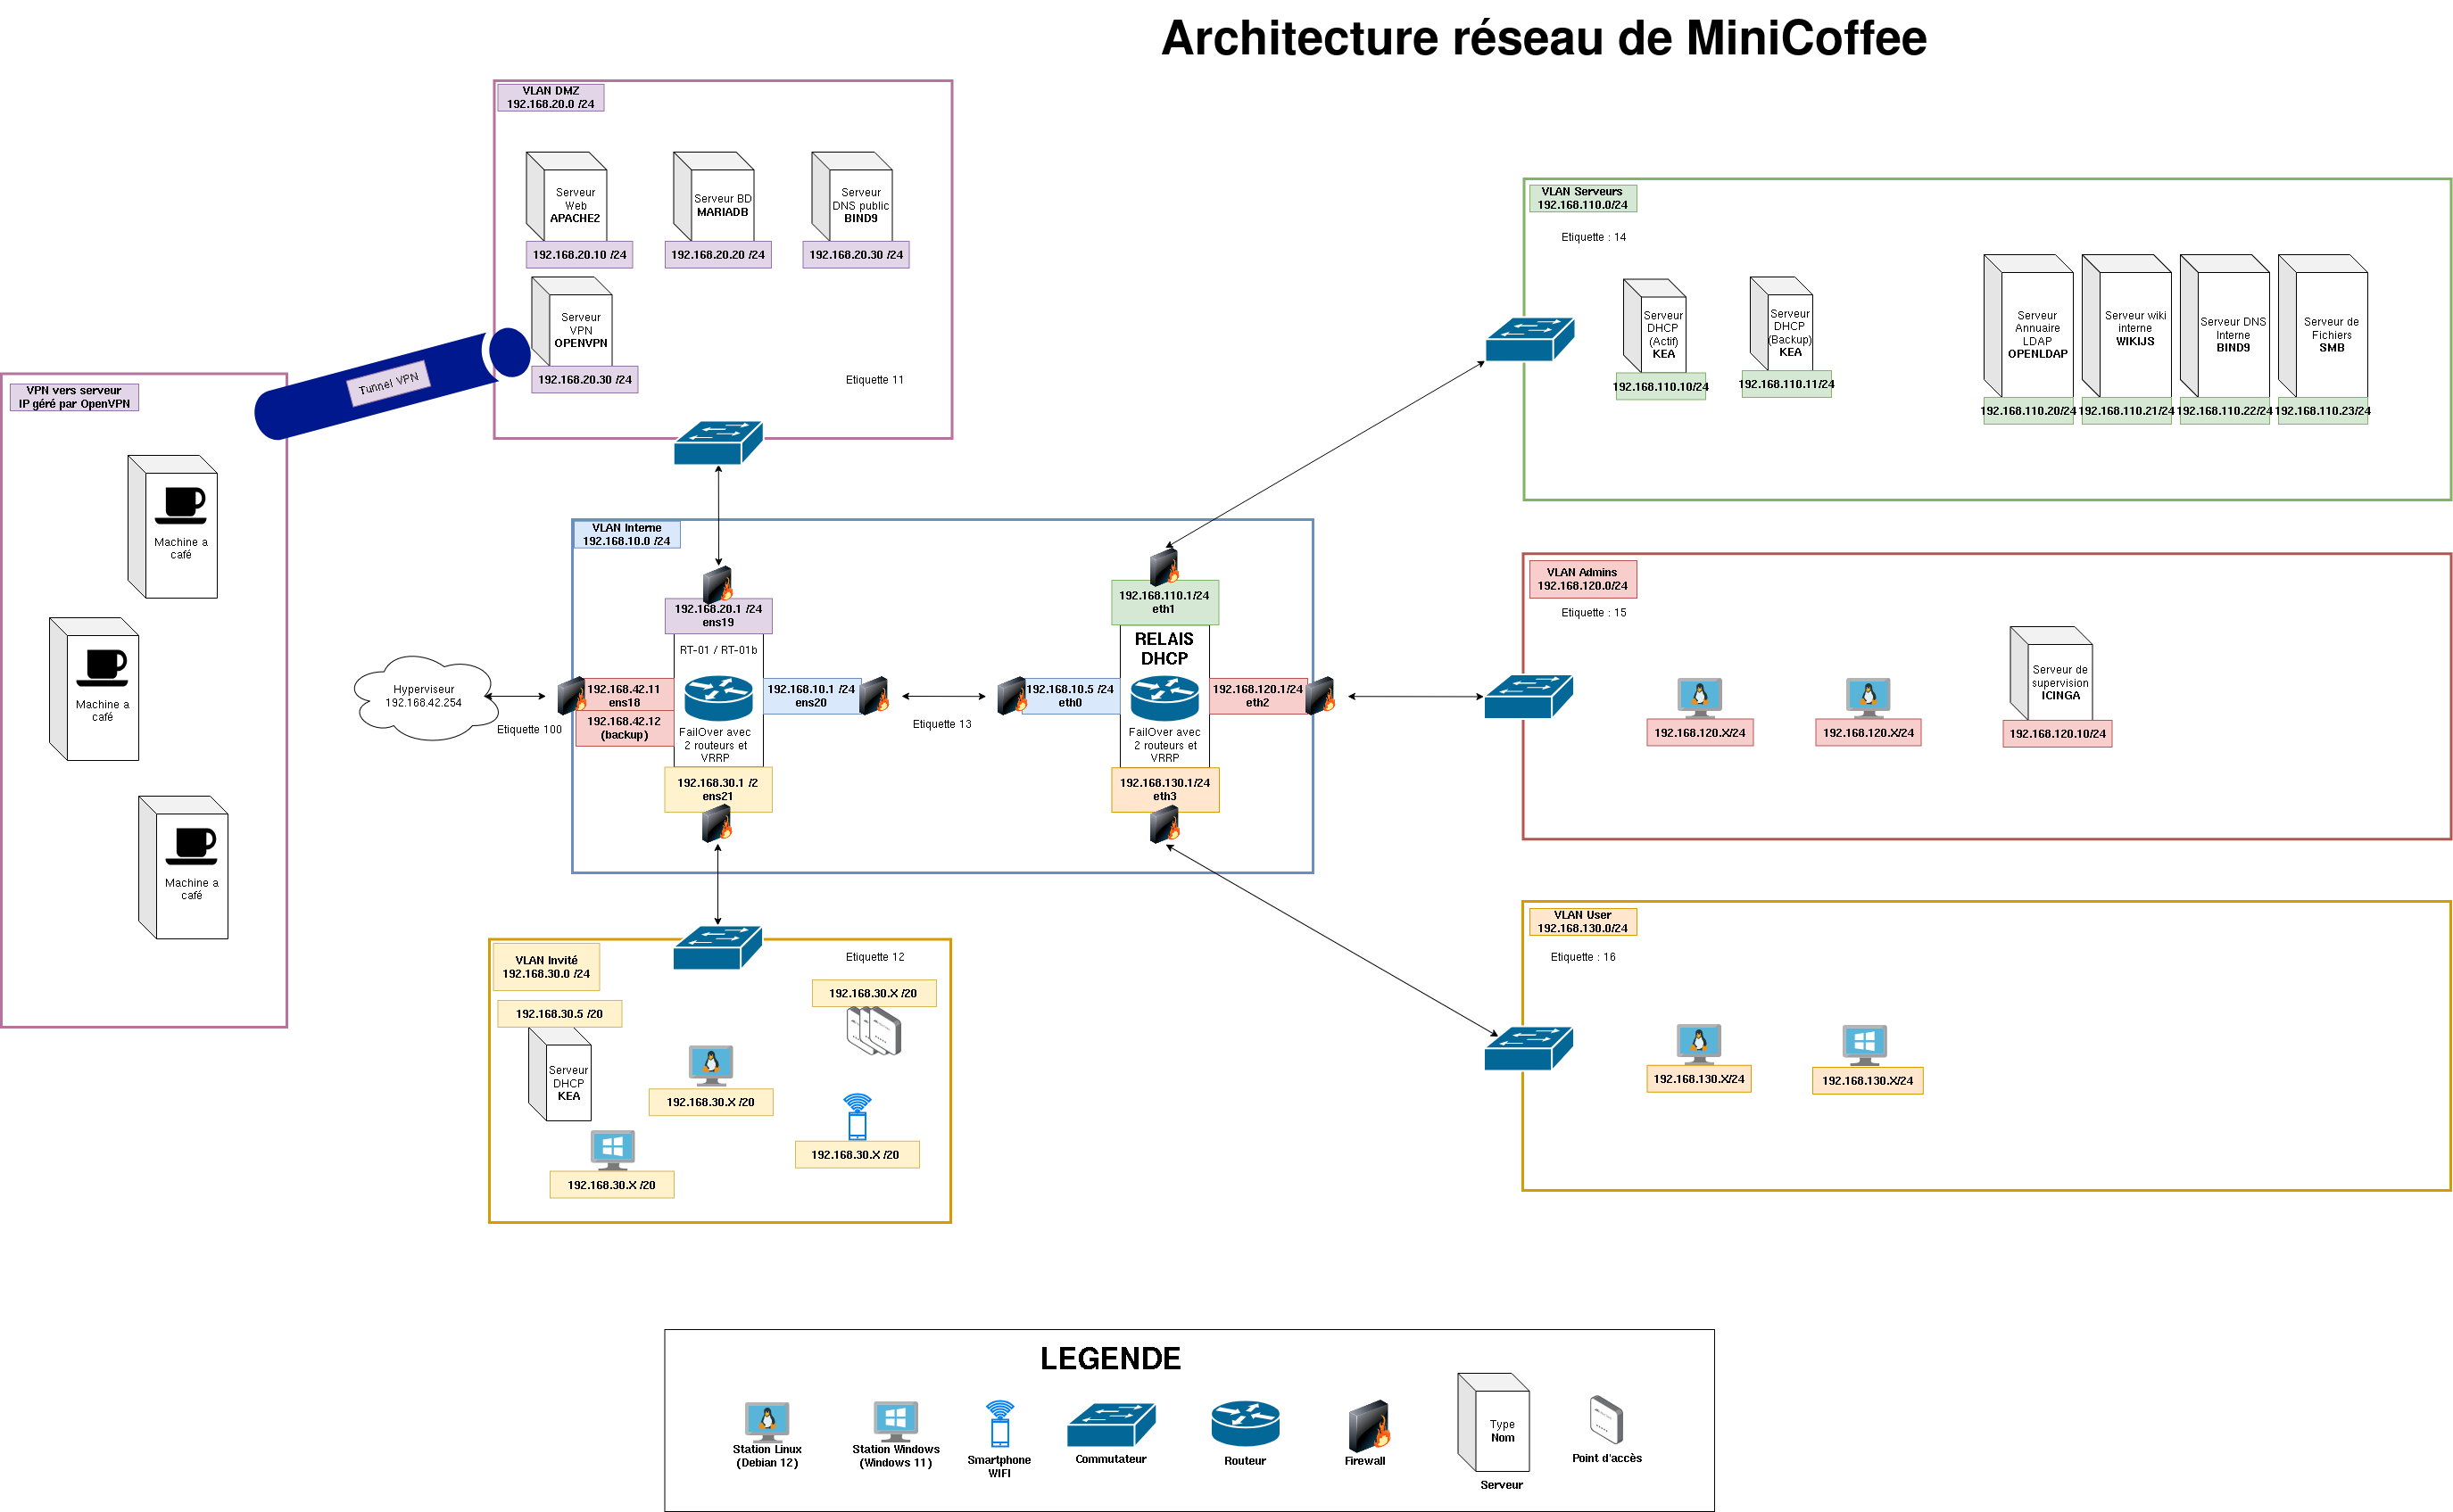
\includegraphics[angle=-90, width=1\textwidth, trim=0 0 0 2.3cm, clip]{../assets/Architecture.drawio.png}
    \caption{Architecture réseau de MiniCoffee}
\end{figure}

\clearpage

\section{Ressources Matérielles utilisées}
Actuellement, notre infrastructure réseau comprend un total de 9 machines actives, chacune jouant un rôle spécifique dans notre environnement.
\\

En ce qui concerne le stockage, nous allouons entre 3 et 5 Go d’espace disque par machine, en fonction de leurs besoins en ressources et des tâches qu’elles doivent accomplir. Plus précisément :
\begin{itemize}
    \item Les machines nécessitant le moins de ressources se voient attribuer 3 Go de stockage, ce qui est suffisant pour assurer leur bon fonctionnement sans surconsommation d’espace.
    \item Les machines les plus sollicitées, qui traitent des volumes de données plus importants ou exécutent des processus plus intensifs, bénéficient quant à elles de 5 Go de stockage afin de garantir des performances optimales.
\end{itemize}

En termes de mémoire vive (RAM), chaque machine de notre réseau dispose actuellement de 1 Go. Cette allocation permet de répondre aux besoins de nos applications tout en maintenant un bon équilibre entre performance et consommation de ressources.
\\

Nous surveillons régulièrement l’utilisation de la RAM et du stockage afin d’optimiser notre infrastructure si nécessaire et d’anticiper toute montée en charge.

\section{Installation et Configuration des éléments de l'infrastrucure}
Nous allons détailler dans cette partie comment nous avons configuré les éléments de notre infrastructure réseau.
\subsection{Résaux Virtuel}

Nous avons créé des VXLAN pour interconnecter les hyperviseurs au sein du cluster, permettant ainsi une communication entre eux. De plus, nous avons mis en place des VNET spécifiques pour chaque hyperviseur afin de segmenter et d’optimiser la gestion du réseau virtuel, garantissant une meilleure performance et une isolation accrue des ressources.

\subsection{Routeurs}
\subsubsection{Configuration des interfaces}
Tout d'abord, il faut configurer les interfaces de la machine qui va servir de routeur.

Il faut configurer le fichier \textbf{/etc/network/interfaces} pour attribuer les bonnes ip et CIDR pour chaque interface. Voici un explique de chaque paramètre que l’on peut mettre :

\newpage



Voici un fichier de configuration type pour un routeur avec plusieurs interfaces :

\begin{configbox}{/etc/network/interfaces}
    \begin{lstlisting}
# Interface WAN (connectee a Internet)
auto eth0
iface eth0 inet 
mtu 1450  # Taille MTU standard
# Interface LAN 1 
(reseau interne 192.168.1.0/24)
auto eth1
iface eth1 inet static
    address 192.168.1.1/24
    gateway 192.168.1.254  
    # Facultatif, utilise uniquement si ce reseau doit 
    sortir par une autre route
    dns-nameservers 192.168.1.1 8.8.8.8
    dns-domain lan1.local
    mtu 1450  # Optimise pour les reseaux 
    locaux rapides

# Interface LAN 2 
(reseau interne 10.10.0.0/24)
auto eth2
iface eth2 inet static
    address 10.10.0.1/24
    mtu 1450  # Optimise pour un second 
    reseau local

# Activation du routage entre les reseaux
post-up echo 1 > /proc/sys/net/ipv4/ip_forward

# Ajout de routes pour permettre aux deux reseaux de communiquer entre eux
post-up ip route add 192.168.1.0/24 via 192.168.1.1 dev eth1 
post-up ip route add 10.10.0.0/24 via 10.10.0.1 dev eth2 
    \end{lstlisting}
\end{configbox}
\paragraph{Détail de la configuration}
\begin{itemize}
    \item Une première ligne avec la façon d’on l’interface s’active.
    \begin{itemize}
        \item (L2) \monosp{auto [nomInterface]}  : Pour activer automatiquement au démarrage. Idéal pour les interfaces fixes, comme celles des serveurs.
        \item \monosp{allow-hotplug [nomInterface]} : Pour activer uniquement quand elle est détectée. Idéal pour les interfaces amovibles.
    \end{itemize}
    \item Une seconde qui définit sa configuration.
    \begin{itemize}
        \item \monosp{iface eth0 inet manual} : Interface n'a pas de configuration IP et doit être activé à la main
        \item \monosp{iface eth0 inet none} : Interface active mais sans configuration IP
        \item (L3) \monosp{iface [nomInterface] inet dhcp} : Utilise le DHCP pour l'attribution d'IP, ...
        \item (L8) \monosp{iface eth1 inet static} : Pour faire une configuration avec une IP statique
    \end{itemize}
    \item Ajout de paramètres pour la configuration de IP si configuration \monosp{static} :
    \begin{itemize}
        \item (L9) \monosp{address 192.168.1.1/24} : L'adresse IP static
        \item (L10) \monosp{gateway 192.168.1.254} : Le gateway
        \item (L13) \monosp{dns-nameservers 192.168.1.1 8.8.8.8} : Les DNS
        \item (L14) \monosp{dns-domain lan1.local} : Le domaine DNS
        \item \monosp{metric 10} : La priorité de l'utilisation de cette interface. Plus la valeur est basse, plus la priorité est haute.
        \item \monosp{up ip addr add 192.168.100.15/24 dev [nomInterface]} : Si l'on souhaite plusieurs adresses IP sur la même interface
        \item (L4) \monosp{mtu 1450} : MTU maximum
        \item (L33) \monosp{post-up ip route add 192.168.1.0/24 via 192.168.100.10} : Si la machine doit accéder à un réseau via une passerelle spécifique. Tout le trafic vers 192.168.200.0/24 passera via 192.168.100.10.
    \end{itemize}
\end{itemize}

Une fois le fichier configuré, il redémarrer le service avec 
\rootcmd{systemctl restart networking.service}

\subsubsection{Configuration des routes entre les réseaux}

Pour permettre au routeur principal de rediriger correctement le trafic destiné aux sous-réseaux internes (hébergés derrière un second routeur), nous avons configuré l’interface réseau avec des routes statiques. Cela permet au système d’orienter les paquets vers le bon « next-hop » (le routeur intermédiaire).

Cette configuration est définie dans le fichier \texttt{/etc/network/interfaces} à l’aide du mot-clé \texttt{up}, qui exécute les commandes au moment où l’interface devient active.

Voici un exemple de configuration pour l’interface \texttt{ens20}, qui est connectée au réseau interne~:

\begin{configbox}{/etc/network/interfaces}
\begin{lstlisting}
allow-hotplug ens20
iface ens20 inet static
        address 192.168.10.2/24
        # ici config ...
        # Pour le routeur 2
        up ip route add 192.168.110.0/24 via 192.168.10.5
        up ip route add 192.168.120.0/24 via 192.168.10.5
        up ip route add 192.168.130.0/24 via 192.168.10.5
\end{lstlisting}
\end{configbox}

\begin{itemize}
  \item \texttt{allow-hotplug ens20}~: Active automatiquement l'interface lorsque le câble réseau est branché.
  \item \texttt{iface ens20 inet static}~: Définit une adresse IP statique pour l'interface.
  \item \texttt{address 192.168.10.2/24}~: Adresse IP attribuée à cette interface (appartenant au réseau \texttt{192.168.10.0/24}).
  \item \texttt{up ip route add ...}~: Ajoute manuellement des routes statiques pour atteindre les réseaux \texttt{192.168.110.0/24}, \texttt{192.168.120.0/24} et \texttt{192.168.130.0/24} via le routeur intermédiaire \texttt{192.168.10.5}.
\end{itemize}

Sans cette configuration, le routeur ne saurait pas comment atteindre ces réseaux via l'autre routeur.

\subsubsection{NAT et règles de pare-feu sur un routeur}

Le pare-feu et la traduction d’adresses (NAT) sont essentiels au fonctionnement sécurisé du routeur. Nous avons configuré ces éléments à l’aide de \textbf{nftables}, qui remplace iptables dans les systèmes Linux récents.

\paragraph{Structure des fichiers~:}

Le fichier principal \texttt{/etc/nftables.conf} agit comme point d’entrée pour charger l’ensemble des règles. Son contenu est minimal et se contente d’inclure des fichiers spécialisés~:

\begin{configbox}{/etc/nftables.conf}
\begin{lstlisting}[language=bash]
#!/usr/sbin/nft -f

flush ruleset

include "/etc/nftables/ruleset/sets.nft"
include "/etc/nftables/ruleset/filter.nft"
include "/etc/nftables/ruleset/nat.nft"
include "/etc/nftables/ruleset/logging.nft"
\end{lstlisting}
\end{configbox}

\paragraph{Organisation modulaire :}
\begin{itemize}
  \item \texttt{sets.nft} contient tous les groupes d'adresses IP (DMZ, LAN, invités, etc.).
  \item \texttt{filter.nft} contient les règles de filtrage (input, output, forward).
  \item \texttt{nat.nft} gère la traduction d'adresse (masquerade vers Internet).
  \item \texttt{logging.nft} contient les chaînes pour journaliser proprement les paquets rejetés.
\end{itemize}

\paragraph{Mécanisme de NAT :}

Le routeur 1 agit comme passerelle vers Internet. Pour permettre aux machines internes d'accéder à Internet, il faut faire du NAT (masquage)~:

\begin{configbox}{nat.nft}
\begin{lstlisting}
table ip nat {
    chain prerouting {
        type nat hook prerouting priority dstnat;
        policy accept;
    }

    chain postrouting {
        type nat hook postrouting priority srcnat;
        policy accept;
        oifname "ens18" masquerade
    }
}
\end{lstlisting}
\end{configbox}

Ici, toutes les connexions sortant via l'interface WAN \texttt{ens18} seront masquées, permettant aux machines internes d’utiliser l’IP publique du routeur.

\paragraph{Filtrage par zones :}

Le pare-feu distingue les interfaces selon les zones (WAN, DMZ, LAN, invités) et applique une politique stricte de contrôle~:

\begin{itemize}
    \item \textbf{INPUT} : seuls le SSH depuis des IP précises et le protocole VRRP sont autorisés.
    \item \textbf{FORWARD} : contrôle précis des flux inter-réseaux.
    \item \textbf{OUTPUT} : le routeur ne génère que le minimum de trafic (DNS, ICMP, VRRP).
    \item \textbf{IPv6} : toutes les connexions IPv6 sont bloquées (table \texttt{ip6 filter\_ipv6}).
\end{itemize}

\paragraph{Fichier avec les règles du routeur 1:}

Ci-dessous, les règles nftables du routeur 1~:

\begin{configbox}{/etc/nftables.config}
\begin{lstlisting}
table inet filter {
        chain input {
                type filter hook input priority filter; policy drop;
                ip version != 4 drop
                iifname "lo" accept
                ct state established,related accept
                ip protocol vrrp ip daddr 224.0.0.18 accept
                iifname { "ens18", "ens19" } ip saddr @ip_ssh_autorise tcp dport 22 ct state new jump log_input_ssh
                jump log_input_unknown
        }

        chain output {
                type filter hook output priority filter; policy drop;
                ct state established,related accept
                ip protocol icmp icmp type echo-request accept
                ip daddr 224.0.0.18 ip protocol vrrp accept
                udp dport 53 ct state new accept
        }

        chain forward {
                type filter hook forward priority filter; policy drop;
                ct state established,related accept
                iifname "ens18" oifname "ens19" ip daddr 192.168.20.10 tcp dport { 80, 443 } ct state new accept
                iifname "ens19" oifname "ens20" ip saddr @dns_clients ip daddr 192.168.110.22 udp dport 53 ct state new accept
                iifname "ens20" oifname "ens18" ct state new accept
                iifname "ens20" oifname "ens19" ip daddr @dmz_net ct state new accept
                iifname "ens19" oifname "ens18" ip saddr @dmz_net ct state new accept
                iifname "ens19" oifname "ens20" ip saddr @dmz_net ip daddr @internal_net jump log_forward_dmz_to_lan
                iifname "ens19" oifname "ens21" ip saddr @dmz_net ip daddr @guest_net jump log_forward_dmz_to_guest
                iifname "ens21" oifname "ens18" ip saddr @guest_net ct state new accept
                iifname "ens21" ip saddr @guest_net ip daddr 192.168.30.10 udp sport 68 udp dport 67 accept
                oifname "ens21" ip saddr 192.168.30.10 ip daddr @guest_net udp sport 67 udp dport 68 accept
                iifname "ens21" ip saddr @guest_net ip daddr @guest_net jump log_guest_to_guest_block
                iifname "ens21" ip daddr @all_internal_net jump log_forward_guest_to_lan
                jump log_forward_unknown
        }
}
table ip6 filter_ipv6 {
        chain input {
                type filter hook input priority filter; policy drop;
        }

        chain forward {
                type filter hook forward priority filter; policy drop;
        }

        chain output {
                type filter hook output priority filter; policy drop;
        }
}

\end{lstlisting}
\end{configbox}


\paragraph{Log structuré~:}

Toutes les actions de rejet sont journalisées via des chaînes spécifiques (ex.~: \texttt{log\_input\_unknown}, \texttt{log\_forward\_dmz\_to\_lan}) ce qui permet un débogage efficace.

\subsubsection{Haute disponibilit\'e avec Keepalived avec le routeur}

Afin d’assurer la tolérance aux pannes et la continuité de service réseau, nous avons mis en place un mécanisme de \textit{haute disponibilité} (HA) entre deux routeurs à l’aide de l’outil \textbf{Keepalived}. Cette solution repose sur le protocole \textbf{VRRP} (Virtual Router Redundancy Protocol) qui permet de partager une IP virtuelle entre plusieurs machines redondantes.

\paragraph{Principe de fonctionnement :}
Tout repose sur la configuration d'un fichier~:\ avec Keepalived, on choisit un \textbf{routeur actif (MASTER)} et un autre de secours (\textbf{BACKUP}). Le routeur actif gère l’IP virtuelle (VIP) utilisée par les clients comme passerelle. En cas de défaillance du MASTER (ex. perte d’interface, arrêt du service), le BACKUP avec la priorité suivante prend automatiquement le relais.

\paragraph{Architecture mise en place :}
Deux routeurs sont configurés :
\begin{itemize}
  \item \textbf{RT-01-Master}~: MASTER avec une priorité élevée, détient la VIP
  \item \textbf{RT-01-Backup}~: BACKUP avec une priorité inférieure, prend le relais si le MASTER tombe
\end{itemize}

Une IP virtuelle est utilisée comme passerelle par interface, par exemple~:\ \ip{192.168.30.1/24} pour le LAN Invité.

\paragraph{Configuration de Keepalived :}
Sur chaque routeur, Keepalived est installé via :

\rootcmd{apt install keepalived}

Le fichier principal de configuration est \texttt{/etc/keepalived/keepalived.conf}. Voici un exemple pour l'interface \texttt{ens21} (réseau invité)~:

\begin{configbox}{/etc/keepalived/keepalived.conf}
\begin{lstlisting}
# Script de verification de la sante de nftables
vrrp_script check_nft {
    script "/etc/keepalived/scripts/check_nft.sh"
    interval 3
    fall 2
    rise 3
}

vrrp_instance VI_INVITE {
    state MASTER
    interface ens21
    virtual_router_id 40
    priority 100
    advert_int 1
    authentication {
        auth_type PASS
        auth_pass "mdp"
    }
    virtual_ipaddress {
        192.168.30.1/24
    }
    track_interface {
        ens21
    }
    track_script {
        check_nft
    }
    notify_master "/etc/keepalived/scripts/notify_vrrp.sh MASTER ens21"
    notify_backup "/etc/keepalived/scripts/notify_vrrp.sh BACKUP ens21"
    notify_fault  "/etc/keepalived/scripts/notify_vrrp.sh FAULT ens21"
}
\end{lstlisting}
\end{configbox}

\paragraph{Analyse de la configuration :}
\begin{itemize}
  \item \textbf{L2}~: Déclare un bloc de supervision \texttt{vrrp\_script} nommé \texttt{check\_nft}.
  \item \textbf{L3}~: Définit le chemin du script qui vérifie si le pare-feu nftables est correctement chargé.
  \item \textbf{L4}~: Le script est exécuté toutes les 3 secondes.
  \item \textbf{L5}~: Si deux échecs consécutifs ont lieu, on considère que l’état est défaillant.
  \item \textbf{L6}~: Il faut trois vérifications réussies pour revenir à un état sain.
  \item \textbf{L10}~: Ce routeur démarre comme MASTER.
  \item \textbf{L11}~: Interface réseau concernée (\texttt{ens21}).
  \item \textbf{L12}~: Identifiant unique de l’instance pour éviter les collisions.
  \item \textbf{L13}~: Priorité élevée (100), donc ce routeur est favorisé.
  \item \textbf{L15--L18}~: Bloc d’authentification VRRP avec mot de passe partagé.
  \item \textbf{L19--L21}~: Attribution de l’adresse virtuelle \texttt{192.168.30.1} à cette interface.
  \item \textbf{L22--L24}~: Vérifie que l’interface réseau est active.
  \item \textbf{L25--L27}~: Supervision du bon fonctionnement de nftables grâce au script \texttt{check\_nft}.
  \item \textbf{L28--L30}~: Déclenche des scripts selon le changement d’état VRRP (MASTER, BACKUP, FAULT).
\end{itemize}

Sur le routeur BACKUP, seul le champ \texttt{state MASTER} devient \texttt{state BACKUP}, et la \texttt{priority} est diminuée (par exemple \texttt{priority 90}). Une instance VRRP est configurée par interface réseau.

\paragraph{Fichiers de scripts et de journalisation :}
Les changements d'état (MASTER, BACKUP, FAULT) déclenchent des scripts dans \texttt{/etc/keepalived/scripts/}. Ces scripts journalisent les transitions dans \texttt{journalctl} au format JSON lisible par un SIEM~:

\begin{itemize}
  \item \texttt{notify_vrrp.sh}~: reçoit en argument l'état et l'interface, et logue un message structuré.
  \begin{codebox}{/etc/keepalived/scripts/notify_vrrp.sh}
	\begin{lstlisting}[language=Bash]
#!/bin/bash

STATE="$1"
INTERFACE="$2"
HOST=$(hostname)
TIMESTAMP=$(date -Is)

# Verifie que les deux arguments sont bien fournis
if [ -z "$STATE" ] || [ -z "$INTERFACE" ]; then
  echo "[ERROR] Usage: $0 <STATE> <INTERFACE>" >&2
  exit 1
fi

# Recupere la VIP secondaire associee a l'interface passee
VIP=$(ip -o addr show dev "$INTERFACE" | awk '/secondary/ {print $4}' | head -n1)

# Log structure en JSON dans journalctl
logger -t KEEPALIVED \
  "{\"event\":\"VRRP\",\"router\":\"$HOST\",\"state\":\"$STATE\",\"interface\":\"$INTERFACE\",\"vip\":\"$VIP\",\"timestamp\":\"$TIMESTAMP\"}"
	\end{lstlisting}
  \end{codebox}
	
  \item \texttt{check_nft.sh}~: vérifie que \texttt{nft list ruleset} renvoie un jeu de règles non vide.
\end{itemize}

\paragraph{Avantages obtenus :}
\begin{itemize}
  \item Continuité d’accès au réseau même si le routeur principal tombe
  \item Pas de changement d’adresse IP pour les clients (VIP fixe)
  \item Récupération automatique sans intervention manuelle
  \item Logs compatibles avec Wazuh
\end{itemize}


\subsection{Serveur DHCP}
Afin de pouvoir attribuer des @IP de façon automatique, nous allons installer un serveur DHCP, le logiciel que nous allons utiliser pour le DHCP s'appelle \monosp{Kea}. Kea est un serveur DHCP développé par l'ISC, conçu pour être plus flexible et performant que ISC DHCP. Kea supporte IPv4 et IPv6 et est particulièrement adapté aux environnements à grande échelle nécessitant une gestion avancée des adresses IP

\subsubsection{Installation}
\begin{itemize}
    \item Nous créons une VM avec une @IP statique car c’est cette dernière qui attribuera les @IP.
    \item Installation de Kea : \rootcmd{apt install kea-dhcp4-server}
\end{itemize}

\subsubsection{Configuration}
\begin{itemize}
    \item Nous sauvegardons la configuration pour la restaurer en cas de problème 
    \rootcmd{mv /etc/kea/kea-dhcp4.conf /etc/kea/kea-dhcp4.conf.bkp}
    \item Nous créons par la suite le fichier \monosp{/etc/kea/kea-dhcp4.conf} qui doit contenir la configuration suivante :
\end{itemize}
    \newpage
\begin{configbox}{/etc/kea/kea-dhcp4.conf.bkp}
    \begin{lstlisting}
{
"Dhcp4": {
	"interfaces-config": {
		"interfaces": [
			"ens18"
		]
	},
	"valid-lifetime": 691200,
	"renew-timer": 345600,
	"rebind-timer": 604800,
	"authoritative": true,
	"lease-database": {
		"type": "memfile",
		"persist": true,
		"name": "/var/lib/kea/kea-leases4.csv",
		"lfc-interval": 3600
	},
	"subnet4": [
		{
			"subnet": "192.168.120.0/24",
			"pools": [
				{
					"pool": "192.168.120.10 - 192.168.120.200"
				}
			],
			"option-data": [
				{
					"name": "domain-name-servers",
					"data": "192.168.110.22"
				},
				{
					"name": "domain-search",
					"data": "bav4.local"
				},
				{
					"name": "routers",
					"data": "192.168.120.1"
				}
			]
		},
[... Ajouter autant de subnet que de sous reseaux sont concernes]
	]
}
}
    \end{lstlisting}
\end{configbox}
\paragraph{Détail de la configuration}
\begin{itemize}
	\item (L2) \monosp{"Dhcp4"} : Indique que l'attribution est faite avec des @IPv4
	\item (L3-5) Indique l'interface qui emettra les DHCP response
	\item (L8-11) Configuration des differents temps de sauvegarde/renouvellement...
	\item (L12-17) Configuration de la base de donnée qui contiendras les données DHCP
	\item (L18) \monosp{"subnet4"} : Indique que le subnet spécifié est en IPv4
	\item (L20) \monosp{ "subnet": "192.168.14.0/24"} : indique le sous reseau ou le serveur DHCP attribue les adresses.
	\item (L21-26) Configure les differents intervalles IP attribués
	\item (L27-L39) Configure les options DHCP (@IP du serveur DNS, adresse du serveur DNS, @IP du routeur)
\end{itemize}

\subsubsection{Ajout d'un relais DHCP}

Dans notre réseau, il nécessaire de permettre à des clients situés dans des sous-réseaux différents d'obtenir une configuration IP automatique à partir d’un serveur DHCP centralisé. Pour cela, nous avons mis en place un relais DHCP (\textit{DHCP relay}) sur le routeur (routeur 2 dans notre cas) assurant l’interconnexion des réseaux.

\paragraph{Configuration utilisée :}
Le paquet utilisé est \texttt{isc-dhcp-relay}, installé sur le routeur. La commande d’installation est la suivante :

\rootcmd{apt install isc-dhcp-relay}

Il faut ensuite adapté le fichier de configuration \monosp{/etc/default/isc-dhcp-relay} avec les paramètres suivants :

\begin{itemize}
  \item \textbf{SERVERS} : adresse IP du serveur DHCP, par exemple \texttt{192.168.110.11}
  \item \textbf{INTERFACES} : interfaces du routeur à écouter (ex. \texttt{ens19, ens20, ens21})
\end{itemize}

\begin{configbox}{/etc/default/isc-dhcp-relay}
\begin{lstlisting}
# What servers should the DHCP relay forward requests to?
SERVERS="192.168.110.11"

# On what interfaces should the DHCP relay (dhrelay) serve DHCP requests?
INTERFACES="ens19 ens20 ens21"
\end{lstlisting}
\end{configbox}

\begin{itemize}
	\item (L2) Adresse IP du serveur DHCP Kea
	\item (L5) Ici les interfaces sur lequels le serveur DHCP va pour être relayer.
\end{itemize}

\paragraph{Résultat attendu :}
Grâce à cette configuration, les clients présents dans les sous-réseaux reliés à \texttt{ens19}, \texttt{ens20} et \texttt{ens21} peuvent désormais obtenir dynamiquement leur adresse IP à partir du serveur DHCP, même s’ils ne sont pas directement connectés à lui.

\subsection{Serveur DNS}
Afin de pouvoir lier un nom a une machine, nous allons installer des serveurs DNS (Domain Name Server), ces derniers feront le lien entre les @IP des différentes machines et le nom que nous leur avons attribué. Le logiciel en charge du DNS s'appelle \monosp{BIND 9}. BIND 9 est un serveur DNS open source développé par l’ISC. Il est reconnu pour sa stabilité, sa sécurité et sa compatibilité avec les standards du DNS. Doté de nombreuses fonctionnalités avancées, il prend en charge DoT (DNS over TLS), le contrôle d’accès, la journalisation fine, ainsi que la gestion en mode maître/esclave. BIND 9 est configurable via des fichiers texte et s’adapte aussi bien aux petits réseaux qu’aux infrastructures de grande taille

\paragraph{Marche a suivre :}
\begin{enumerate}
	\item Nous allons créer 2 serveur DNS, un serveur Externe, qui va être accessible depuis l’exterieur, et un serveur DNS Interne, qui va être accessible uniquement depuis l’interieur, ca sera utile pour le wiki. 
	\item Nous allons commencer par créer le DNS privé puis nous le cloneront pour en faire un DNS public, il faudra juste supprimer les alias créés pour le wiki, supprimer l’ACL “lan” et l’option lan dans allow-query (voir suite)
\end{enumerate}

\subsubsection{Installation de BIND9}
Nous installons Bind9 via apt avec la commande suivante :
\rootcmd{apt install bind9 dnsutils}

\subsubsection{Configuration des options DNS}
Nous allons d'abord copier la configuration pour pouvoir la rétablir facilement en cas d'erreur :
\rootcmd{cd /etc/bind }
\rootcmd{cp named.conf.options named.conf.options.bkp}
\rootcmd{cp named.conf.local named.conf.local.bkp} 

Nous allons ensuite modifier le fichier de config \monosp{/etc/bind/named.conf.options} qui contient les options du serveur DNS.	
\begin{configbox}{/etc/bind/named.conf.options}
\begin{lstlisting}
acl "lan" {
	192.168.110.0/24;
	192.168.120.0/24;
	192.168.130.0/24;
	localhost;
	localnets;
};
options{ 
	forwarders{
		152.77.1.22
	}
	allow-query { lan; }; 
};
\end{lstlisting}
\end{configbox}
\paragraph{Détail de la configuration}
\begin{itemize}
	\item (L1) \monosp{acl "lan"} : On déclare une ACL appellée "lan", qui permet que seule les @Ip spécifiées auront accès au serveur DNS
	\item (L2-7) Déclarations des sous-réseaux concernés par l'ACL
	\item (L9-11) On change le forwarder (le serveur DNS qui résoudra les noms si le nôtre ne les contient pas) par le DNS de l'UGA
	\item (L12) \monosp{allow-query { lan; };} indique que seuls les sous-réseaux de l'ACL peuvent query le serveur DNS
\end{itemize}

\subsubsection{Configuration de zone} 
Nous allons desormais créer la zone bav4.local, c'est cette derniere qui contiendra les enregistrements dns (par exemple wiki.bav4.local). Dans \monosp{/etc/bind/named.conf.local}, nous ajoutons donc la zone suivante:

\begin{configbox}{/etc/bind/named.conf.local}
\begin{lstlisting}
zone "bav4.local" {
    type master;
    file "/etc/bind/db.bav4.local";
    allow-update { none; };
};
\end{lstlisting}
\end{configbox}
\paragraph{Détail de la configuration}
\begin{itemize}
	\item (L2) Indique que ce serveur DNS est l'autorité principale (ou maître) pour la zone bav4.local.
	\item (L3) Indique l'emplacement du fichier qui contient les enregistrements (voir suite)
	\item (L4) Interdit toute mise à jour dynamique des enregistrements DNS pour la zone concernée.
\end{itemize}

Nous allons ensuite dupliquer le fichier \monosp{db.local} en l’appellant db.bav4.local pour pouvoir configurer la zone : 
\rootcmd{cp /etc/bind/db.local /etc/bind/db.bav4.local}
Puis, dans \monosp{db.bav4.local}, nous allons mettre en place la config suivante :
\label{subsubsec:confzonedns}
\begin{configbox}{/etc/bind/named.conf.local}
\begin{lstlisting}
$TTL    604800
@       IN     SOA    srv-dns.bav4.local.  root.bav4.local. (
                              1         ; Serial
                         604800         ; Refresh
                          86400         ; Retry
                        2419200         ; Expire
                         604800 )       ; Negative Cache TTL
;
@               IN      NS      srv-dns.bav4.local.
srv-dns         IN      A       192.168.110.22
ldap			IN		A		192.168.110.30

[... ajouter autant d'enregistrement que necessaire]
\end{lstlisting}
\end{configbox}
\paragraph{Détail de la configuration}
\begin{itemize}
	\item (L3) Numéro de serie
	\item (L4) Délai de rafraichissement pour la synchronisation des configurations entre plusieurs serveurs DNS
	\item (L5) Délai au bout duquel un serveur DNS secondaire devra retenter une synchronisation
	\item (L6) Temps d'expiration du serveur DNS
	\item (L7) Durée de conservation dans le cache de l'information "NXDOMAIN"
	\item (L9-LXX) Création des enregistrement DNS : plusieurs formes possibles :
	\begin{enumerate}
		\item \textbf{Lien nom-@IP :}	<nom-de-l'hote>   	IN	A		<@IP>
		\item \textbf{Lien alias-nom :}	<nom-de-l'alias> 	IN	CNAME 	<nom-de-l'enregistrement-de-référence>
	\end{enumerate}		  
\end{itemize}

Une fois cela fait, relançons \monosp{bind9} et notre serveur DNS est maintenant opérationnel :
\rootcmd{systemctl restart bind9}
\rootcmd{systemctl enable named.service}

Pour le vérifier, utilisons la commande suivante :
\cmd{nslookup google.com}

\subsubsection{Configuration de DoT (DNS over TLS}
Afin de rajouter une couche de sécurité dans les requetes DNS, nous allons utiliser DoT (DNS over TLS) qui permet de chiffrer nos requetes DNS. Nous utiliseront par la suite \monosp{systemd-resolved} du coté client.

\paragraph{Niveau Serveur\\}
\monosp{bind9 v9.18.33} supporte DoT sans besoin d'un logiciel tiers de type proxy, nous allons donc le mettre en place directement dans bind9.
\begin{enumerate}
	\item Nous créons et se place dans un nouveau dossier \monosp{ssl}
\rootcmd{cd /etc/bind/ssl}
	\item Nous générons une clé et un certificat (auto-signé), nécessaires pour TLS :
\rootcmd{openssl req -x509 -newkey rsa:2048 -nodes -keyout /etc/bind/ssl/cleDNS.key -out /etc/bind/ssl/certDNS.crt -days 365 -subj "/CN=bav4.local"
}
	\item Nous donnons ensuite l'ownership de la clé a \monosp{bind}
\rootcmd{chown bind:bind /etc/bind/ssl/cleDNS.key}
	\item Finalement, nous modifions le fichier de configuration \monosp{/etc/bind/named.conf.options}, vu précédemment : 
	\begin{configbox}{/etc/bind/named.conf.options}
		\begin{lstlisting}
tls servertls {
	cert-file "/etc/bind/ssl/certDNS.crt";
	key-file "/etc/bind/ssl/cleDNS.key";
};
options {
[...]

	listen-on { any; };
	listen-on-v6 { any; };
	listen-on tls servertls { any; };
	allow-query { lan; };

}
		\end{lstlisting}
	\end{configbox}
	\paragraph{Détail de la configuration}
	\begin{itemize}
		\item (L1) Déclaration d'un bloc tls "\monosp{servertls}"
		\item (L2-3) Indique le chemin vers le certificat et la clé
		\item (L10) Indique que le serveur écoute les requêtes TLS liées au blocs \monosp{servertls} sur toutes les adresses (restreintes en réalités a l'ACL "lan" vu précédemment)
	\end{itemize}
\end{enumerate}

\paragraph{Niveau Client\\}

Pour utiliser DoT facilement sur les machines client, nous allons utiliser le package \monosp{systemd-resolved} :

\begin{enumerate}
	\item Nous installons systemd-resolved : \rootcmd{apt install systemd-resolved}
	\item Nous allons ensuite modifier la configuration de ce dernier :
\begin{configbox}{/etc/systemd/resolved.conf}
\begin{lstlisting}
[...]

[Resolve]
DNS=192.168.110.24#bav4.local
DNSOverTLS=yes

[...]
\end{lstlisting}
\end{configbox}
\paragraph{Détail de la configuration}
\begin{itemize}
	\item (L4) Déclaration du DNS qui va être utilisé (\ip{192.168.110.24}) et son hostname (bav4.local), spécifié lors de la création du certificat vu plus haut dans ce document
	\item (L5) Activation le mode DNSOverTLS
\end{itemize}
	\item Nous copions ensuite le certificat DNS \monosp{certDNS.crt} présent sur le serveur DNS :
\rootcmd{scp SERVDNS:/etc/bind/ssl/certDNS.crt /usr/local/share/ca-certificates/certDNS.crt}
	\item Puis, nous rechargeons les certificats avec : \rootcmd{update-ca-certificates}
	\item Finalement, dans \monosp{/etc/nsswitch.conf}, nous changeons la ligne \monosp{hosts} :  
\begin{configbox}{/etc/nsswitch.conf}
\begin{lstlisting}
[...]
hosts:	files	resolve	dns
[...]
\end{lstlisting}
\end{configbox}
la ligne \monosp{hosts} a donc 3 options, ainsi:
\begin{enumerate}
	\item Le système vérifie le fichier local \monosp{/etc/hosts}, cette methode est très rapide
	\item Si cela échoue, le système va tenter d'utiliser \monosp{systemd-resolved}
	\item Si cela échoue, le système interroge directement un serveur DNS configuré via \monosp{/etc/resolv.conf}
\end{enumerate}
\end{enumerate}

Finalement, nous testons si resolvectl fonctionne avec :
\rootcmd{resolvectl status}
Et la résolution de nom (chiffrée) avec 
\rootcmd{resolvectl query google.com}

Pour automatiser cette configuration, nous allons modifier les machines templates pour que les prochaines VMs utilisent DoT et créer un script d'automatisation d'installation pour les machines déja existantes.

\paragraph{Script a éxécuter sur les machines client\\}
\begin{codebox}{scriptDoTClient.sh}
\begin{lstlisting}[language=Bash]
#!/bin/

# Definir l'adresse IP du serveur DNS et son nom de domaine
DNS_IP="192.168.110.24"
DNS_HOSTNAME="monserveur.local"

echo "Installation de systemd-resolved..."

apt update && apt install -y systemd-resolved

# Activer et demarrer systemd-resolved
systemctl enable --now systemd-resolved

echo "systemd-resolved est installe et actif."

# Sauvegarde des fichiers avant modification
echo "Sauvegarde des fichiers de configuration..."
cp /etc/systemd/resolved.conf /etc/systemd/resolved.conf.bak
cp /etc/nsswitch.conf /etc/nsswitch.conf.bak
echo "Changement de la config"
rm /etc/nsswitch.conf
rm /etc/systemd/resolved.conf
cp /tmp/nsswitch.conf /etc/nsswitch.conf
cp /tmp/resolved.conf /etc/systemd/resolved.conf
cp /tmp/certDNS.crt /usr/local/share/ca-certificates/certDNS.crt

echo "Update du certificat"
update-ca-certificates

# Redemarrer systemd-resolved pour appliquer les changements
echo "Redemarrage de systemd-resolved..."
systemctl restart systemd-resolved

# Tester la resolution DNS
echo "Test de resolution DNS avec systemd-resolved..."
if resolvectl query google.com | grep -q "google.com"; then
    echo "Test reussi : la resolution DNS fonctionne"
    echo "Configuration terminee !"
else
    echo "Echec du test DNS. Verifie la configuration."
fi
\end{lstlisting}
\end{codebox}
\paragraph{Détail du script}
\begin{itemize}
	\item (L4-5) Déclaration de l'@IP du serveur DNS et le nom du certificat
	\item (L9-12) Installation et activation de \monosp{systemd-resolved}
	\item (L18-19) Sauvegarde des anciens fichiers de configuration
	\item (L21-23) Remplacement de la configuration
	\item (L24) Ajout du certificat
	\item (L28) Update des certificats
	\item (L32) Redemarrage de \monosp{systemd-resolved}
	\item (L36-40) Test de connectivité final
\end{itemize}

\newpage

\paragraph{Script a éxécuter sur \monosp{Bastion}\\}
Ce script nécéssite que la machine Bastion ait les fichiers \monosp{nsswitch.conf}, \monosp{resolve.conf}, \monosp{scriptDoTClient.sh} dans le répertoire dans lequel ce trouve le script.

\begin{codebox}{scriptDoTServeur.sh}
\begin{lstlisting}[language=Bash]
#!/bin/bash
for host in m1 m2 m3 m4; do
    scp scriptDoTClient.sh nsswitch.conf resolved.conf certDNS.crt $host:/tmp/
    ssh $host
done
\end{lstlisting}
\end{codebox}
A chaque connection, nous effectuerons en plus la commande \cmd{su -c /tmp/scriptDoTClient.sh}
\paragraph{Détail du script}
\begin{itemize}
	 \item (L1) Itération dans différentes machines connues par \monosp{Bastion}
	 \item (L2) Copie des fichiers nécessaires
	 \item (L3) Ouverture d'une liaison ssh
\end{itemize}


\subsection{Wiki}

Pour le wiki nous avons comparé plusieurs choix, on a choisi Wiki.js pour plusieurs raisons essentielles.
Tout d’abord, Wiki.js est simple à installer et à administrer, tout en étant très puissant. Il fonctionne avec une base de données (PostgreSQL, MySQL, etc.), ce qui permet une gestion efficace du contenu. Son interface utilisateur moderne et intuitive facilite la navigation et la rédaction des pages.
Ensuite, Wiki.js offre une gestion avancée des permissions, ce qui permet de contrôler précisément qui peut voir ou modifier les pages. Il prend aussi en charge plusieurs formats d’édition, dont Markdown, facilitant ainsi la contribution des utilisateurs.
Enfin, il est open-source, léger et extensible grâce à ses nombreux modules. Il permet aussi l’intégration avec Git, ce qui est un gros avantage pour la collaboration et la gestion des versions du wiki.

\subsubsection{Installation/Configuration de WikiJS}

\paragraph{Prérequis\\}

\begin{enumerate}
	\item Nous allons commencer par installer les packages \monosp{curl}, \monosp{software-properties-common},  \monosp{postgreSQL}, \monosp{node.js} :
\rootcmd{apt install -y curl software-properties-common}
\rootcmd{curl -fsSL https://deb.nodesource.com/setup_18.x | sudo -E bash - }
ajoute le dépôt de Node.js 18 sur une distribution Debian ou Ubuntu et préparer l’installation de Node.js à partir des packages officiels de NodeSource.
\rootcmd{apt install -y nodejs postgresql}
	\item On se connecte ensuite la base postgres : \cmd{su -i -u postgres psql}
	\item On crée la base wikijs et l'utilisateur postgres wikiuser :
	\begin{codebox}{shell postgres}
\begin{lstlisting}
CREATE DATABASE wikijs;
CREATE USER wikiuser WITH ENCRYPTED PASSWORD 'motdepasse';
GRANT ALL PRIVILEGES ON DATABASE wikijs TO wikiuser;
\q
\end{lstlisting}
\end{codebox}
\end{enumerate}

\paragraph{Installation/configuration\\}
\begin{enumerate}
	\item Nous installons wikijs et le serveur node.js :
\cmd{mkdir /var/www/wikiJS \&\& cd /var/www/wikiJS}
\cmd{curl -fsSL https://get.requarks.io/wiki/latest.tar.gz | tar xz -C .}
télécharge et extrait la dernière version de Wiki.js dans le répertoire courant.
\cmd{npm install}
	
	\item Nous allons ensuite modifier la configuration \textbf{/var/www/wikiJS/config.yml}
	\begin{configbox}{/var/www/wikiJS/config.yml}
	\begin{lstlisting}
db:
  type: postgres
  host: localhost
  port: 5432
  user: wikiuser
  pass: motdepasse
  db: wikijs
	\end{lstlisting}
	\end{configbox}
	\begin{itemize}
		\item (L2) specifie le type de base de données
		\item (L3) specifie quel serveur heberge la base de données
		\item (L4) Port utilisé pour la base de données
		\item (L5) Nom d'utilisateur de la base de données
		\item (L6) Mot de passe de l'utilisateur de la base de données
		\item (L7) Nom de la base de données
	\end{itemize}
	
	\item Finalement, démarrons Wiki.js :
	\cmd{node server}
\end{enumerate}

\subsubsection{Configuration de Nginx comme Proxy}
Nous allons maintenant configurer un Proxy avec Nginx pour signé le wiki et avoir un accès HTTPS.

\paragraph{Installation\\}
Nous installons nginx via apt :
\rootcmd{apt install nginx}
\paragraph{Configuration du Virtual Host\\}

\begin{enumerate}
	\item Nous allons d'abord générer le certificats est la clé pour pouvoir signer le wiki
\rootcmd{sudo mkdir -p /etc/ssl/private /etc/ssl/certs
sudo openssl req -x509 -nodes -days 365 -newkey rsa:4096 \
    -keyout /etc/ssl/private/wiki-js-key-no-pass.pem \
    -out /etc/ssl/certs/wiki-js-cert.pem}
	\item Créons un fichier de configuration :
\rootcmd{nano /etc/nginx/sites-available/wiki}
	\item Dans ce dernier, ajoutons le contenu suivant :
\begin{configbox}{/etc/nginx/sites-available/wiki}
\begin{lstlisting}
	server {
		listen 80;
		server_name 192.168.110.47;
		return 301 https://$host$request_uri;
	}
	
	server {
		listen 443 ssl;
		server_name 192.168.110.47;
	
		ssl_certificate "/etc/ssl/certs/wiki-js-cert.pem";
		ssl_certificate_key "/etc/ssl/private/wiki-js-key-no-pass.pem";
	
		ssl_protocols TLSv1.2 TLSv1.3;
		ssl_ciphers 'HIGH:!aNULL:!MD5';
	
		location / {
			proxy_pass http://192.168.110.21:3000;
			proxy_http_version 1.1;
			proxy_set_header Upgrade $http_upgrade;
			proxy_set_header Connection 'upgrade';
			proxy_set_header Host $host;
			proxy_cache_bypass $http_upgrade;
		}
	}
\end{lstlisting}
\end{configbox}
\begin{itemize}
	\item (L2) port sur lequel tourne le proxy
	\item (L3) adresse ip de la machine qui heberge le proxy
	\item (L4) Redirige toutes les requêtes HTTP vers HTTPS en utilisant une redirection permanente (301).
	\item (L8) Écoute sur le port 443 (HTTPS) et active SSL.
	\item (L11) Chemin vers le certificat SSL utilisé pour sécuriser la connexion.
	\item (L12) Clé privée associée au certificat SSL.
	\item (L14) Autorise uniquement TLS 1.2 et 1.3 (plus sécurisés).
	\item (L15) Autorise uniquement TLS 1.2 et 1.3 (plus sécurisés).
	\item (L18) Redirige les requêtes vers Wiki.js qui tourne sur 192.168.110.21:3000.
	\item (L19) Utilise HTTP/1.1, nécessaire pour les connexions WebSocket.
	\item (L20) Gère les WebSockets (indispensable pour certaines fonctionnalités).
	\item (L21) Indique que la connexion doit être mise à niveau (pour WebSockets).
	\item (L22) Transmet l’hôte original demandé par le client.
	\item (L23) Désactive la mise en cache si un Upgrade est demandé (important pour les WebSockets).
\end{itemize}
	\item On active ensuite la configuration :
	\rootcmd{ln -s /etc/nginx/sites-available/wiki /etc/nginx/sites-enabled/}
	\rootcmd{systemctl restart nginx}
\end{enumerate}


\subsubsection{Accès interne}
Pour acceder au wiki depuis n'importe quel station interne, il va falloir au préalable l'inscrire dans les enregistrement de notre serveur DNS : \underline{\ref{subsubsec:confzonedns}}


\subsection{SIEM}

\subsubsection{Installation de Wazuh}
\begin{enumerate}
	\item Ajout du dépôt Wazuh
	\rootcmd{curl -sO <https://packages.wazuh.com/key/GPG-KEY-WAZUH>}
	Cette commande utilise curl pour télécharger la clé GPG publique de Wazuh, ce qui permet au système de vérifier l’authenticité des paquets de Wazuh lors de leur installation. 
	\rootcmd{apt-key add GPG-KEY-WAZUH}
	Ajoute la clé GPG téléchargée au gestionnaire de paquets APT pour valider les paquets provenant du dépôt Wazuh.
	\rootcmd{echo 'deb <https://packages.wazuh.com/4.x/apt/> stable main' | tee /etc/apt/sources.list.d/wazuh.list}
	Ajoute le dépôt Wazuh à la liste des sources d’APT, ce qui permet au système d’installer des paquets depuis ce dépôt.
	\rootcmd{apt update}

	\item Installation du serveur Wazuh
	\rootcmd{apt install wazuh-manager}
	\rootcmd{systemctl enable --now wazuh-manager}
	Active et démarre immédiatement le service wazuh-manager pour qu’il fonctionne au démarrage du système.
\end{enumerate}

\subsubsection{Installation de l'Elastic Stack}

\begin{enumerate}
	\item Installation d'Elasticsearch
	\rootcmd{wget -qO - https://artifacts.elastic.co/GPG-KEY-elasticsearch | apt-key add -}
	Télécharge et ajoute la clé GPG de l’Elastic Stack afin de valider les paquets d’Elasticsearch.
	\rootcmd{echo "deb https://artifacts.elastic.co/packages/8.x/apt stable main" | tee -a /etc/apt/sources.list.d/elastic-8.x.list}
	Ajoute le dépôt officiel d’Elasticsearch à la liste des sources APT pour que le système puisse télécharger et installer Elasticsearch
	\rootcmd{apt update \&\& apt install elasticsearch}
	\rootcmd{systemctl enable --now elasticsearch}

	\item Installation de Kibana
	\rootcmd{apt install kibana}
	\rootcmd{systemctl enable --now kibana}

\end{enumerate}

\subsubsection{Configuration de Filebeat sur le routeur}
On configure Filebeat sur une machine pour pouvoir envoyer des informations(logs, traffic réseaux...) au SIEM.

\begin{enumerate}
	\item Installation de Filebeat
	\rootcmd{apt install filebeat}

	\item Configuration de Filebeat pour Elasticsearch et Kibana
	\begin{configbox}{/etc/filebeat/filebeat.yml}
		\begin{lstlisting}
filebeat.inputs:
- type: log
  enabled: true
  paths:
    - /var/log/*.log

output.elasticsearch:
  hosts: ["<http://192.168.110.23:9200>"]
  username: "elastic"
  password: "enamont"
setup.kibana:
  host: "<http://192.168.110.23:5601>"

		\end{lstlisting}
	\end{configbox}

	\begin{itemize}
		\item (L1) Specification des fichiers a envoyer au SIEM
		\item (L2) Type des fichiers envoyées
		\item (L4) Chemin vers les fichiers à envoyées
		\item (L8) URL vers l'interface elasticsearch
		\item (L9) username utilisé pour se connecter à elasticsearch
		\item (L10) Mot de passe utilisé pour se connecter à elasticsearch
		\item (L12) URL pour acceder à kibana
	\end{itemize}

	\item Activation du module Netflow
	\rootcmd{filebeat modules enable netflow}
	Module qui permet d'enregistrer le traffic réseaux
	\rootcmd{systemctl restart filebeat}


	
\end{enumerate}



\end{document}